% Sources primaires

\subsection{L’astronomie ptoléméenne : naissance et diffusion}
    \subsubsection{\textit{L'Almageste} et le modèle ptoléméen}
	L'astronomie et les disciplines qui y sont liées sont, dès l'Antiquité, cultivées dans un grand nombre de cultures où se développent des pratiques variées, appuyées sur l'observation des objets célestes et le développement de systèmes mathématiques pour en prédire le comportement. Jusqu'à l'arrivée des théories de Nicolas Copernic au \xv siècle, les travaux de Ptolémée\footnote{Claude Ptolémée (v. 100-v. 170) est un astronome, mathématicien et géographe actif à Alexandrie au \ii siècle de notre ère. \textit{L'Almageste}, complété vers 150, comprend un quart de siècle d'observations des mouvements des objets célestes, expliqués par des systèmes mathématiques qu'il développe dans son œuvre. Le système ptoléméen désigne le modèle géocentrique de l'univers qu'il développe dans ses travaux. \cite{jonesPtolemya}.} influencent, à travers l'Eurasie, les productions des astronomes. L'œuvre de Ptolémée devient en effet dès le \ii siècle une référence en matière d'astronomie : développées sur les travaux de ses prédécesseurs grecs, les théories de Ptolémée approfondissent les productions de son temps dont il fait la synthèse dans ses travaux, et qu'il enrichit de ses propres observations. Si le modèle géocentrique est déjà établi avant l'achèvement de \textit{L'Almageste}, les travaux de Ptolémée perfectionnent la théorie des épicycles\footnote{Introduite par les astronomes de la Grèce antique, la théorie des épicycles permet, dans un modèle géocentrique, d'expliquer les changements de vitesse et de direction dans le mouvement observé des planètes, du Soleil et de la Lune. Selon cette théorie, les objets célestes se déplacent à vitesse uniforme sur un cercle appelé épicycle, dont le centre est lui-même en rotation sur un cercle centré sur la Terre appelé déférent. \cite{rousseauEpicyclesPtolemee}}, et parviennent à l'affiner avec une précision suffisante pour la prédiction des positions des planètes, notamment par l'introduction du point équant\footnote{En effet, la théorie des épicycles telle qu'elle existe avant l'intervention de Ptolémée ne permet pas de justifier précisément des mouvements observés des planètes. Ptolémée introduit ainsi la notion de point équant, point excentré par rapport au centre de la Terre, à partir duquel la vitesse de rotation des corps céleste est constante. Ce modèle géométrique permet de calculer avec précision le mouvement longitudinal des planètes. \cite{evansHistoryAstronomy}}.
	
	\textit{L'Almageste} est constitué d'observations et descriptions des procédures mathématiques appliquées par Ptolémée pour établir les paramètres de son modèle géométrique\footcite{evansHistoryAstronomy}. À ses explications textuelles s'ajoutent des tables de valeurs numériques calculées par Ptolémée qui permettent, en suivant ses explications, de calculer la position des planètes, en tant qu'application de ses théories. Dans les siècles qui suivent le développement du modèle ptoléméen, peu d'innovations ont lieu dans les sciences astronomiques de tradition hellénique, et les travaux produits prennent essentiellement la forme de commentaires des théories de Ptolémée, sans remise en cause de son modèle, qui reste la norme pendant plusieurs siècles et est diffusé à travers l'Eurasie par le biais de traductions.

    \subsubsection{Diffusion du modèle ptoléméen}
	Avant les Grecs, les Babyloniens pratiquent, dès le \ist millénaire \jc, une astronomie basée sur des calculs arithmétiques permettant de prédire la position des planètes. L'astronomie indienne hérite de ces théories des sciences astronomiques babyloniennes qu'elle mêle avec des méthodes locales, qui s'enrichissent plus tard des travaux de Ptolémée et de son prédécesseur Hipparque, dont les idées voyagent vers l'Est\footcite{evansHistoryAstronomy} par le biais de la Perse.
	
	À partir du \viii siècle, dans le monde islamique, se développe une pratique de l'astronomie à l'intersection des théories grecques, babyloniennes, perses et indiennes. Suivant le modèle des tables de Ptolémée, les astronomes arabes développent au \ix siècle des ouvrages de tables, appelés \textit{zīj}, dédiés au calcul des positions du Soleil, de la Lune et des planètes mêlant ces diverses traditions. La traduction en arabe -- pendant le califat abbasside\footnote{La dynastie sunite des Abbassides gouverne le monde musulman de 750 à 1258. La capitale du califat, Bagdad, est le siège d'entreprises de traduction vers l'arabe d'écrits scientifiques, notamment depuis le grec.} -- des écrits de Ptolémée permet aux astronomes du monde islamique d'enrichir leurs pratiques en l'inscrivant dans cette tradition, tout en améliorant certains paramètres calculés dans le cadre de son modèle pour en préciser les prédictions\footnote{L'écart temporel entre les calculs de Ptolémée et ceux des astronomes arabes du \ix siècle permettent également de mettre en évidence certains déplacements observables seulement sur un temps plus long, tels que la diminution de l'obliquité de l'écliptique.}. Si des critiques des travaux de Ptolémée émergent, notamment au \xie siècle dans les écrits d'Ibn al-Haytham, son modèle reste prédominant jusqu'aux travaux de Copernic\footcite{evansHistoryAstronomy}.
	
	Dans le monde latin, les théories grecques se sont peu transmises, et l'enseignement de l'astronomie s'appuie essentiellement sur les écrits de Pline l'Ancien. Au \xii et \xiii siècles, les textes grecs sont rendus disponibles par des initiatives de traduction : Gérard de Crémone, notamment, traduit \textit{L'Almageste}\footnote{Ainsi que d'autres versions arabes de textes grecs, tels que \textit{Du ciel} d'Aristote, ou les \textit{Éléments} d'Euclide.} de l'arabe vers le latin, participant activement à la redécouverte du modèle ptoléméen par les scientifiques du monde latin. La transmission des écrits et théories astronomiques ne se fait donc pas directement des Grecs aux Latins, mais a pour intermédiaires les traductions effectuées aux siècles prédécents dans le monde arabo-musulman. En parallèle, le développement des universités réintègre l'astronomie à l'enseignement des arts libéraux : dans ce contexte d'émulation, de nouveaux ouvrages sont publiés, et notamment des tables astronomiques, toujours basés sur le modèle ptoléméen.
	
	Les sources chinoises témoignent d'une pratique de l'astronomie aussi ancienne que le \ii millénaire \jc sous la forme de prédiction des éclipses du Soleil et de la Lune. Cette pratique est profondément liée à la culture impériale, et les éclipses -- puis plus tardivement, les planètes -- sont un outil d'analyse du règne d'un empereur. Plus proche des procédures babyloniennes que du modèle géométrique grec, l'astronomie chinoise s'appuie avant tout sur l'arithmétique pour ses prédictions, et s'intéresse principalement aux événements ponctuels -- tels que les comètes ou les éclipses -- plutôt qu'aux mouvements des corps célestes\footcite{evansHistoryAstronomy}.
	
	Jusqu'à l'émergence du modèle héliocentrique, et la mise au centre de la pratique des théories de Copernic, le modèle ptoléméen représente, dans de nombreux contextes culturels, le socle des méthodes des sciences astronomiques. Qu'il soit amélioré, contesté, ou enrichi de pratiques locales, il reste un standard de la conception de l'astronomie en Eurasie, et permet ainsi de retracer une tradition des pratiques à travers les siècles.

\subsection{Les diagrammes}
    \subsubsection{Une culture visuelle des sciences astronomiques}
	Dans le contexte eurasiatique, les supports détaillant les pratiques des astronomes circulent entre les siècles et les cultures, et sont enrichis ou adaptés aux pratiques autochtones de l'astronomie, en réponse aux besoins spécifiques de chaque contexte culturel. Les manuscrits et imprimés, supports de ces pratiques, sont les témoins de ces échanges intellectuels et permettent d'établir une histoire des idées et des méthodes héritées du modèle ptoléméen (fig. \ref{fig:modeles_lune}). Ces œuvres comprennent, en support des pratiques, des textes, des tables et des diagrammes, tous porteurs des méthodes et théories des sciences astronomiques : le projet \dishas ayant mené une étude sur les tables astronomiques, il semble naturel qu'\eida, dans la continuité de celui-ci, ait pour vocation de s'intéresser spécifiquement aux diagrammes. Les astronomes, dans leur pratique, n'hésitent pas à employer des modes d'expression visuels, au-delà du texte, qu'il convient d'étudier en parallèle de celui-ci pour en comprendre les interactions. Ainsi, il est nécessaire de développer des outils permettant d'appréhender les formes variées que peuvent prendre les sources en histoire de l'astronomie ; à l'image des récentes recherches en histoire des sciences, qui s'appliquent notamment à une étude des sources visuelles, non-discursives, de la pratique scientifique, et en considérant les illustrations comme des objets d'étude à part entière, au-delà d'un simple accompagnement du contenu textuel\footnote{\cite{jardineCriticalEditingEarlyModern2010}, p. 394}.
	
	En tant que vecteurs d'une culture visuelle de l'astronomie, les diagrammes sont, pour les astronomes, le support d'une pratique scientifique, et sont ainsi révélateurs de leurs méthodes, de leur contexte d'exercice et de leur conception de ces disciplines. Le projet vise à proposer une analyse de ces diagrammes qui souligne la variété de leurs fonctions et des traditions auxquelles ils appartiennent, tout en étudiant leurs modes de circulation à travers l'histoire de l'astronomie. Dans la diversité de leurs sphères de création, ces diagrammes reçoivent \og une légitimité en tant qu'instruments pédagogiques et vecteurs de la pensée\footnote{\og [...] legitimacy as instruments of pedagogy and as vehicle of thought \fg. \cite{hamburgerDiagramParadigmCrossCultural2022}, p. 1.}  \fg, et occupent ainsi dans le contexte d'une culture visuelle globale une place particulière.

	\begin{figure}[h]
		\begin{subfigure}{0.34\linewidth}
			\centering
			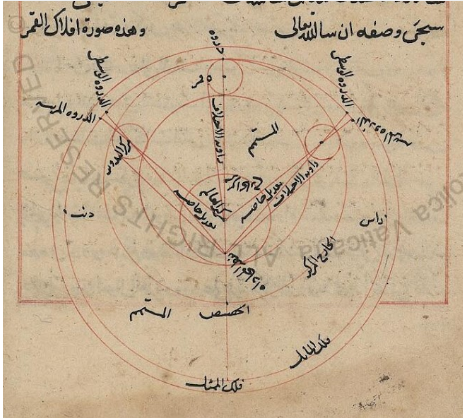
\includegraphics[width=5.5cm]{images/modele_lune_arabe.png}
		\end{subfigure}
		\hspace{1pt}
		\begin{subfigure}{0.30\linewidth}
			\centering
			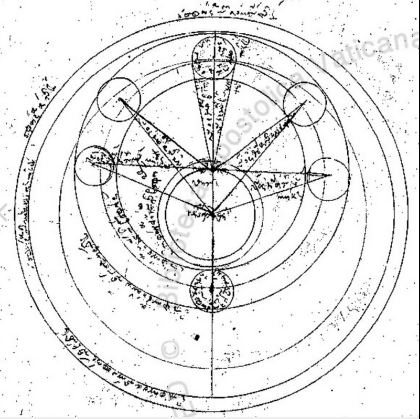
\includegraphics[width=5cm]{images/modele_lune_byz.png}
		\end{subfigure}
  		\hspace{1pt}
  		\begin{subfigure}{0.30\linewidth}
			\centering
			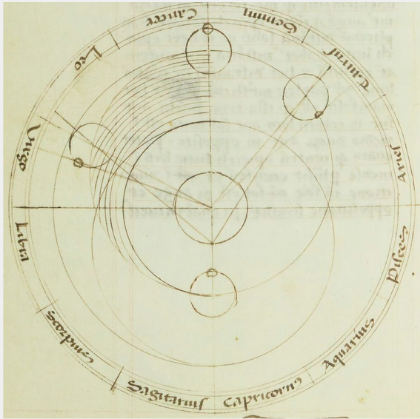
\includegraphics[width=5cm]{images/modele_lune_latin.png}
		\end{subfigure}
		\caption{Diagrammes astronomiques de tradition arabe, byzantine et latine}
		\label{fig:modeles_lune}
	\end{figure}

	\subsubsection{Bornes géographiques et chronologiques}
	Ayant la volonté de produire une étude des circulations et évolutions des diagrammes astronomiques, \eida s'attache à l'étude de sources provenant de sphères géographiques et temporelles larges : les pratiques eurasiatiques des sciences astronomiques partagent des éléments communs qui justifient une étude au cadre vaste, pour proposer une analyse transculturelle des continuités et divergences dans l'histoire de l'astronomie comme dans la culture visuelle. Pour répondre à cette volonté, le projet \eida s'appuie sur cinq corpus aux provenances temporelles et géographiques diverses, provenant de traditions diverses également, dans une volonté de représentativité. 
	
	Les manuscrits astronomiques arabo-persans, produits du \viii au \xviii siècle, représentent à eux seuls un corpus d'une grande diversité, aux traditions diverses aussi bien du point de vue des pratiques que de la provenance géographique. Les travaux produits dans ces contextes circulent à travers l'Eurasie du \ma au début de la période moderne, et influencent de nombreuses pratiques. Les manuscrits d'astronomie latins médiévaux sont produits majoritairement entre le \xiii et le \xvi siècle dans un contexte universitaire, et sont influencés par les traductions faites de l'arabe au latin de textes de tradition arabe ou persane. Les manuscrits byzantins, produits entre les \ix et \xv siècles sont à l'intersection des traditions helléniques, latines et arabo-persanes, et influencent considérablement les manuscrits astronomiques latins du \xv et du \xvi siècle. Les manuscrits sanskrits, dont la diversité reflète les nombreuses traditions établies sur près de deux millénaires, témoignent à partir du \xie siècle d'influences helléniques puis arabo-persanes. Les sources chinoises, dont le support n'est pas nécessairement le manuscrit, prennent souvent la forme d'imprimés par blocs xylographiques dont les matrices sont réemployées à travers plusieurs témoins. Ces documents témoignent des influences arabo-persanes puis latines des pratiques astronomiques chinoises à partir de la dynastie Ming\footnote{La dynastie Ming règne sur la Chine de 1368 à 1644.}. Les sources étudiées dans le cadre d'\eida proviennent essentiellement des dynasties Ming et Qing\footnote{La dynastie Qing, dernière dynastie impériale chinoise, règne de 1644 à 1912.}.
	
	Les bornes de ces cinq corpus représentent les bornes chronologiques et géographiques du projet. S'étendant du \viii au \xviii siècle, les périodes et aides étudiées se veulent représentatives du contexte afro-eurasien de la circulation des idées et des images. Ces corpus représentent, dans chaque cas, plusieurs milliers de manuscrits. Plusieurs centaines de manuscrits sont numérisés pour chaque tradition représentée dans le projet, permettant ainsi la représentativité espérée dans le cadre du projet \eida. Ces numérisations, mises à disposition par les institutions patrimoniales qui conservent ces témoins, représentent les sources primaires du projet, sur lesquelles seront appliquées les traitements en prévision de l'analyse par les chercheurs.
